% !TeX root = ../../thesis.tex

\section{Neither Secure Boot nor BitLocker Enabled}
\label{sec:attacks:neither}

We start by implementing a baseline attack, which we can use to test against Secure Boot and BitLocker and further build upon.
The implementation in the form of a bootkit and a rootkit both share the same approach and core functionality.
The general approach of our attack is to access the Windows installation from within the \ac{UEFI} environment and gain elevated code execution by modifying its contents.

\subsection{Bootkit}
\label{sec:attacks:neither:bootkit}

We start with the description of the bootkit approach.

\subsubsection{Infection}

We have two ways to infect a system: we can either use a bootable medium such as a CD-ROM or a \ac{USB} stick with an \ac{UEFI} application installing the bootkit or we can use a Windows executable.
Booting into the installer application requires either the firmware implementation or the boot order to prefer booting from the removable media over booting Windows directly.
This can be forced during the boot process when accessing the interactive firmware menu at startup, given that it is not password protected.
Installation from Windows requires admin privileges to mount and modify the \ac{ESP}.

The installation process is identical for both options.
We access the \ac{ESP} and create a copy of the Windows Boot Manager located under \program{EFI\textbackslash Microsoft\textbackslash Boot\textbackslash bootmgfw.efi}.
We then replace the original with our bootkit as well as dropping all resources required by the bootkit on the \ac{ESP}.
Now that our bootkit is in place of the Windows Boot Manager, when the \ac{UEFI} Boot Manager selects the boot load option for the Windows Boot Manager, it will cause our bootkit to be executed.
\autoref{fig:windows-boot-entry} shows a dump of the Windows boot entry using the \ac{UEFI} shell command \program{bcfg}.
The entry contains the device path including the file path and optional data.

\begin{figure}[htb]
    \centering
    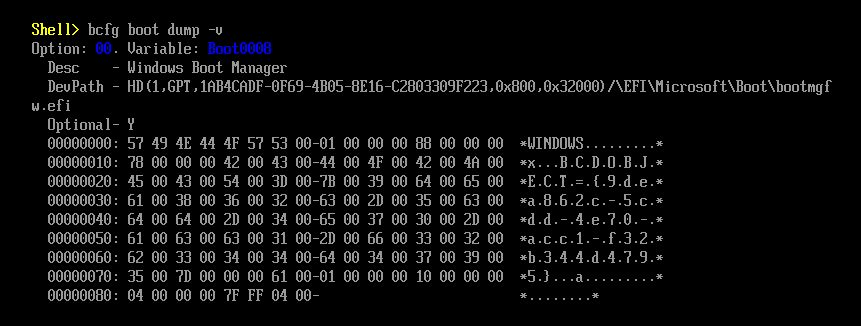
\includegraphics[width=1.0\textwidth]{attacks/neither/windows_boot_entry.png}
    \caption{Windows boot entry, part of the \ac{UEFI} shell output of \program{bcfg}}
    \label{fig:windows-boot-entry}
\end{figure}

\subsubsection{File Access}

The most important step for a storage-based approach is gaining access to the Windows installation from within the \ac{UEFI} environment.
Since \ac{UEFI} does not require the firmware to come with an \ac{NTFS} driver, our attack has to come with its own.
\ac{EDK} II does not provide one, but we can use the open source \ac{NTFS} driver \program{ntfs-3g} from Tuxera \cite{ntfs-3g}.
It was ported to the \ac{UEFI} environment by \emph{pbatard} \cite{ntfs-3g-uefi}.
Using \ac{EDK} II to compile it, we receive a \program{.efi} executable image.

We can use the \ac{UEFI} shell and its file system related commands to test the \ac{NTFS} driver's capabilities.
When booting into the \ac{UEFI} shell we are greeted with a screen displaying the \ac{UEFI} specification version the firmware supports and a list of default mappings for file systems and block devices.
These mappings are created by the shell to provide a short name that can be used interchangeably with a longer device path when issuing commands \cite[Section 3.7.2]{uefi-shell-spec}.
They are designed to be consistent across reboots as long as the hardware configuration stays the same and are comparable to Windows partition letters \cite[Appendix A]{uefi-shell-spec}.
\autoref{fig:mapping} shows the mapping of a partition containing a Windows installation.
As there is no \ac{NTFS} driver present yet, it is only displayed as a block device.

\begin{figure}[htb]
    \centering
    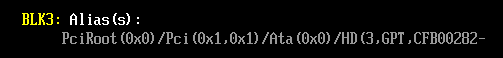
\includegraphics[width=0.8\textwidth]{attacks/neither/mapping}
    \caption{Mapping of the Windows partition}
    \label{fig:mapping}
\end{figure}

We can enter the mapping name of the file system containing our \ac{NTFS} driver to use it as our current working directory and load the driver using the \program{load} command.
The command is executed successfully and the driver is now listed when querying the currently loaded drivers with the command \program{drivers}.
We can now instruct the default mappings to be reset with the \program{map -r} command, to receive an updated list including the file systems now provided through the \ac{NTFS} driver.
\autoref{fig:mapping-ntfs} also shows us that the new file system now sits on top of a device which previously was listed only as a block device.

\begin{figure}[htb]
    \centering
    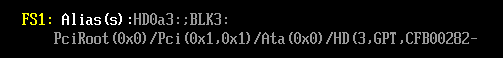
\includegraphics[width=0.8\textwidth]{attacks/neither/mapping_ntfs}
    \caption{Mapping of the mounted Windows partition}
    \label{fig:mapping-ntfs}
\end{figure}

As done before we now type the mapping name of the new file systems, we check the root directories' contents with \program{ls} until we find the partition containing the Windows installation and then enter \program{vol} to check the access rights.
This reveals that the file system is currently read\-/only, as shown in \autoref{fig:vol}.
Upon debugging the \ac{NTFS} driver, it appears to be that the driver falls back to read\-/only when it encounters a file that indicates that the Windows system is in hibernation mode.
We can remove this fallback from the \ac{NTFS} driver's code and recompile.

\begin{figure}[htb]
    \centering
    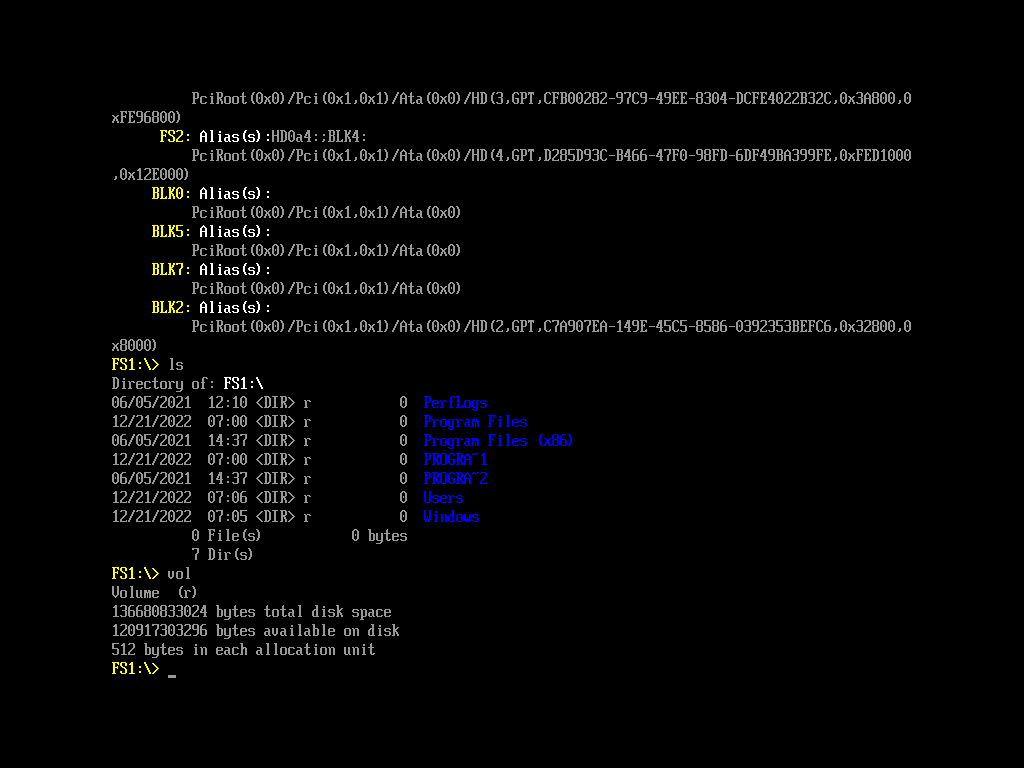
\includegraphics[width=0.5\textwidth]{attacks/neither/vol}
    \caption{Volume Information of the Windows File System}
    \label{fig:vol}
\end{figure}

On the ASRock test setup as described in \autoref{sec:test-setup:asrock}, we noticed that the firmware already shipped with a read\-/only \ac{NTFS} driver included.
In case of our rootkit we would be able to remove this driver by modifying the firmware image, but we can implement a solution that applies to both types of \ac{UEFI} payload.
We can change the \ac{NTFS} driver to install its \nameref{lst:simple-file-system-protocol} under a \ac{GUID} different to the regular \code{gEfiSimpleFileSystemProtocolGuid}.
This enables us to install two instances of the \nameref{lst:simple-file-system-protocol} alongside each other on the same controller.
The alternative \ac{GUID} can then searched for by our root- and bookit, to retrieve our specific protocol instance with write access.
The driver also has to open the protocols it uses without demanding exclusive ownership over them.
This prevents the \ac{NTFS} driver from being denied access, when trying to open a protocol that is already in exclusive ownership \cite[Section 7.3]{uefi-spec}, which would be a likely occurrence as filesystem drivers are encouraged to get exclusive control over their block device \cite[Section 13.5]{uefi-spec}.

We now know that, provided we get to load the \ac{NTFS} driver, we can read and write the files of a Windows installation.
Thus we drop the driver together with the bootkit onto the \ac{ESP} as part of our infection process.
When our bootkit is executed, we use the \nameref{lst:loaded-image-protocol} of our own image handle to retrieve the source device handle from which our bootkit was loaded from \cite[Section 9.1]{uefi-spec}.
As both files reside within the same volume, we can use this handle to call the boot services \code{LoadImage()} and \code{StartImage} to execute the driver.
Since the driver conforms to the \ac{UEFI} driver model, we also need to connect the driver to a device representing the Windows partition using the \nameref{lst:driver-binding-protocol}.
We can do this by retrieving all protocol instances and iterating over all controllers, to connect them recursively.
This way the driver can assume controller over all \ac{NTFS} formatted volumes and install an instance of the \nameref{lst:simple-file-system-protocol} on their handles.

\subsubsection{Payload Deployment}

Before we can deploy our payload we first need to read it into memory.
\code{LoadImage()} is reserved to be used for \ac{UEFI} images.
Non\-/executable files are read directly with the \nameref{lst:simple-file-system-protocol}.
The \ac{ESP}'s device handle can be used with the boot service \code{HandleProtocol()} to retrieve its instance of the \nameref{lst:simple-file-system-protocol}.
A call to \code{OpenVolume()} results in an instance of the \nameref{lst:file-protocol} representing the root folder of the volume \cite[Section 13.4]{uefi-spec}.
The root directory can then be used to open and read our payload with an absolute path.

We need the device handle of the volume containing the Windows installation to perform the write operation.
We can use the boot service \code{LocateHandleBuffer()} to receive an array of all handles that support the \nameref{lst:simple-file-system-protocol}, this includes volumes such as the Windows recovery partition or the \ac{ESP} we just used.
We can iterate over all handles and search for the Windows folder to identify the correct volume.

Now the question arises as to where we write our payload to; our goal here is automatic and elevated execution.
\emph{MosaicRegressor} writes its payload to the Windows startup folder, a folder whose contents are automatically executed at system startup.
The programs within the startup folder are unfortunately not automatically run at an elevated level, so this is not a suitable target location.
We also cannot trivially overwrite or modify executables that are part of the Windows startup process, as \ac{KMCI} will verify their code integrity before execution.

Our approach is to use the \emph{Task Scheduler}.
The Task Scheduler is a Windows service responsible for managing the automatic execution of background tasks \cite[Section 10]{windows-internals-7-part2}.
Tasks are performed on certain triggers, which may be time-based (periodically or at a specific time) or event-based, for example on user logon or system boot \cite{microsoft-task-scheduler-triggers}.
A task can perform various actions upon invocation \cite{microsoft-task-scheduler-actions}.
We will focus on command execution.
Most tasks will simply execute other programs as their action.
This execution is performed under a specified security context \cite{microsoft-task-scheduler-security-contexts}.
The idea is to have a task, that performs its action with a high privilege level, execute our payload.
Our task\-/of\-/choice is called \program{Proxy} and can be found under the \program{Autochk} folder.
Its properties are depicted in \autoref{fig:proxy}.

\begin{figure}[htb]
    \centering
    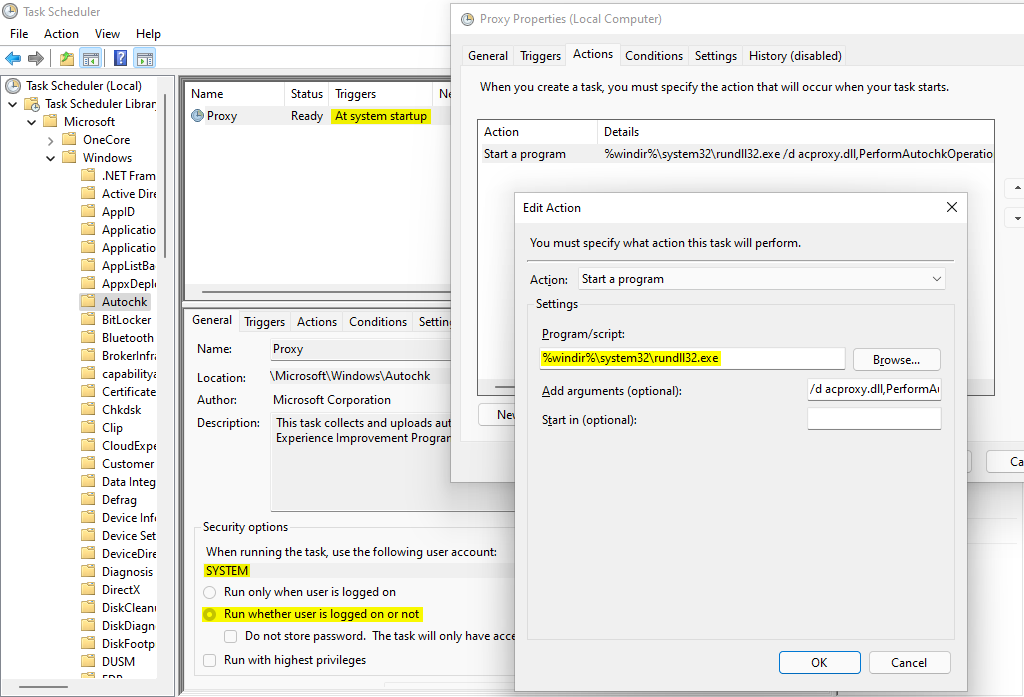
\includegraphics[width=1.0\textwidth]{attacks/neither/proxy}
    \caption{\program{Proxy} Task shown using the Task Scheduler Configuration Tool}
    \label{fig:proxy}
\end{figure}

The \program{Proxy} task is triggered at system startup (with a 30 minute delay) and its action is to start the program \program{rundll32.exe} with the options \code{/d acproxy.dll,PerformAutochkOperations}.
This causes \program{rundll32.exe} to load the \program{acproxy.dll} \ac{DLL} into memory and invoke its exported function \code{PerformAutochkOperations()} \cite{microsoft-rundll32}.
The function name as well as the task name suggest the performed action relates to the Windows utility \program{autochk} which verifies the integrity of \ac{NTFS} file systems \cite{microsoft-autochk}.
Under security options, we can see that the task is executed using the built\-/in \emph{SYSTEM} account.
This task is therefore the perfect candidate to run our payload.

The Task Scheduler keeps book of its active tasks in the Windows registry under the path \program{HKLM\textbackslash SOFTWARE\textbackslash Microsoft\textbackslash Windows NT\textbackslash CurrentVersion\textbackslash Schedule\textbackslash TaskCache}.
The tasks are grouped by four subkeys: \program{boot}, \program{logon}, \program{plain}, and \program{maintenance}.
The entries under these subkeys consist only of a \ac{GUID}.
This \ac{GUID} references the task descriptors that are saved using task master (registry) keys, which are located under \program{HKLM\textbackslash SOFTWARE\textbackslash Microsoft\textbackslash Windows NT\textbackslash CurrentVersion\textbackslash Schedule\textbackslash TaskCache\textbackslash Tasks} \cite[Section 10]{windows-internals-7-part2}.
A secondary copy of the task descriptors exists within the regular file system under \program{\%windir\%\textbackslash system32\textbackslash Task}, stored in the form of \ac{XML} files.

We can use the Task Scheduler Configuration Tool to modify the \program{Proxy} task on a system under our control, changing the executable path as well as remove the delay configured in its trigger.
We can save the output of \program{whoami /all} into a file to verify the privileges our payload is executed with.
The \program{whoami} command shows the current user and privileges \cite{microsoft-whoami}.
After manually triggering the task through the configuration tool, we see that our payload was run from the \emph{nt authority\textbackslash system} user account, which is the most privileged system account \cite{microsoft-localsystem-account}.

\TODO{whoami /all snippet}

Using the Windows registry editor \program{reged.exe} we can navigate to the task descriptor store and search for the task master key belonging to our task.
We can then export the task master key and import it on our victim's system as part of our attack.
By importing an entire registry key, instead of modifying a single value of an existing registry key, the victim's registry keys maintains their integrity, as with a full overwrite the registry key's hash value is also changed.
We can use a Linux utility called \program{chntpw} To import the key.
The tool's primary purpose is to reset the password of local Windows user accounts \cite{chntpw}.
It does this by editing the hive files of a Windows installation and as such the author also offers a standalone registry editor called \program{reged}.
We can test the Linux tool when dual\-/booting Linux and Windows.
For now we place our payload manually in the Windows installation and then boot into Linux, where we can open the \program{HKEY\_LOCAL\_MACHINE/SOFTWARE} hive in \program{reged} and import our modified registry key.
This overwrites the task descriptor and, when booting into Windows, our payload is executed.

Our \ac{UEFI} payload now needs to perform the registry modification from within the \ac{UEFI} environment.
For this we port the \program{reged} utility, so that our bootkit can use it.
The tool is already written in \code{C}, facilitating an easy porting process.
The porting process boils down to providing semantically equivalent definitions for all external functions the program links against.
These functions are mostly \code{C} standard library and Linux kernel related.
Declarations and macros are still supplied by the local compiler's system headers.
We can often use \ac{UEFI} equivalent functions and wrap them to match the required signature.
\ac{EDK} II offers a lot of libraries implementing commonly used abstractions which we can use.
Memory allocation like \code{malloc()} and \code{free()} can be mapped to the \code{MemoryAllocationLib}.
Memory manipulation like \code{memset} and \code{memcpy} to \code{BaseMemoryLib}.
Basic string manipulation like \code{strcmp()} and \code{strlen()} to \code{BaseLib}.
Function calls related to standard input and output such as opening, reading, and writing the hive file, are more complex and have to be mapped to the \ac{UEFI} protocols \nameref{lst:simple-file-system-protocol} and \nameref{lst:file-protocol}.
Luckily the author of \program{reged} used distinct functions to access the hive file and the registry file, making it possible to create the \ac{UEFI} port and keeping the original source code unmodified.

We also make a change to the import behavior, as the name of a task master key is the task's \ac{GUID}.
This may differ from device to device, thus we cannot import a key into its exact path.
We instead iterate over the subkeys of the target's parent key and then match for the name value to find the right key.

Now that we modified the Windows installation to execute our payload upon boot, we need to transfer execution from the bootkit to the original Windows Boot Manager.
Loading the original application is inspired by how the \ac{UEFI} boot manager processes boot options.
This includes relaying the \code{LoadOptions} and \code{ParentHandle} of the \nameref{lst:loaded-image-protocol} from the bootkit's image handle to the Windows Boot Manager's image handle.

\subsection{Rootkit}

Performing the attack in the form of a rootkit is very similar and mainly differs in the infection process.
We now compile the \ac{UEFI} payload as a \ac{DXE} driver instead of a regular \ac{UEFI} application.
When it is placed in a \ac{DXE} volume it is automatically loaded by the \ac{DXE} dispatcher iterating over the \ac{FV}, loading drivers and resolving dependencies.
The core functionality of our \ac{UEFI} payload is identical with the exception that we do not have to manually load the \ac{NTFS} driver anymore and that accessing the Windows payload is now done through the \nameref{lst:firmware-volume2-protocol} defined in the \cite[Section 3.4.1]{pi-spec}, instead of \nameref{lst:simple-file-system-protocol}.
There are no traditional file names in a \ac{FFS}, so we have to search for files using their \acp{GUID}, they are defined within the \ac{EDK} II module file.

\subsubsection{Infection}

Infection with the rootkit has a much higher entry barrier, as it requires read and write access to the firmware image.
\autoref{sec:test-setup} lists how we access the firmware images on our target systems.
But there are also other ways to do this.

\TODO{LIST ALL OPTIONS}
\autoref{sec:past-threats} vector\-/edk potentially exploit \ac{OEM} specific flash mechanism, signing with stolen private key, part of the supply chain, might also be physical \TODO{LIST ALL OPTIONS}

When we are in possession of the image, we need to insert our payload into a \ac{DXE} volume and redeploy the modified image.
We can do this using the previously mentioned \program{UEFITool}, where we navigate to a \ac{DXE} volume, identified by containing \ac{DXE} drivers.
On our \nameref{sec:test-setup:lenovo} system, the firmware image does not contain enough free space to allow for the addition of our payload.
By deleting network drivers, which are not used as Windows is not booted via a network in our attacks, we can debloat the firmware image and insert our drivers.

Our \ac{UEFI} payload in the form of \program{.efi} executable images cannot be directly inserted with \program{UEFITool}, because of the \ac{FFS} file sectioning mentioned in \autoref{sec:ueif-pi:pi:pi-firmware-images}.
\ac{DXE} drivers have three mandatory sections: the \ac{PE32} executable section, composed of the \program{.efi} file content, a version section, and the \ac{DEPEX} section \cite[Vol. 3, 2.1.4.1.4]{pi-spec}.
For our \ac{UEFI} payload to be generated as a sectioned \ac{FFS} file using \ac{EDK} II, we need our drivers to be packaged as part of a \ac{FV}.
We can add our files to the build process of the \ac{OVMF} package in \ac{EDK} II.
The intermediary \program{.ffs} files generated from the build process are of much value for us, as they are the sectioned files we can use in a \ac{FV}.

For our Windows payload we can use a special \ac{EDK} II module type that takes binary files as input.
The generated result is a sectioned file of type \code{EFI\_FV\_FILETYPE\_FREEFORM}.
This type puts no restrictions on the contained file sections \cite[Vol. 3, 2.1.4.1.7]{pi-spec}.
The output contains only one file section of type \code{EFI\_SECTION\_RAW} consisting of the binary payload.

Now that we have \program{.ffs} files corresponding to all our resources used in the attack we can import these into the target image with \program{UEFITool}.
Redeploying the modified image concludes our infection process.

\clearpage
